\subsection{Misura dello Slew Rate}

\begin{wrapfigure}[15]{r}{0.55\textwidth}
  \begin{center}
    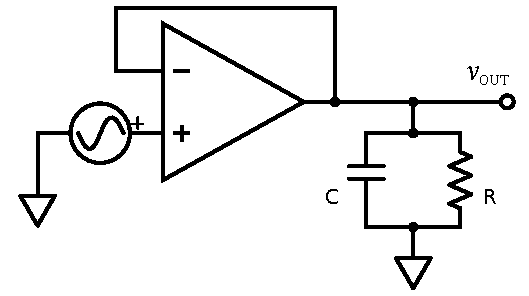
\includegraphics[width=0.30\textwidth]{../E03/latex/slew_rate.pdf}
  \end{center}
  \caption{Schema del circuito utilizzato per stimare lo Slew Rate. La resistenza utilizzata è $R=2.17\pm0.01$\si{\kilo\ohm}; la capacità $C=200 \pm 10$ \si{\pico\farad}.}
  \label{cir3:slew_rate}
\end{wrapfigure}

Uno dei parametri che caratterizzano l'amplificatore operazionale è lo Slew Rate, definito come
$$SR = \frac{\Delta V}{\Delta t}$$
che indica la velocità massima con cui l'amplificatore operazionale può far variare la tensione in uscita nell'unità di tempo. Ciò significa che, per segnali in entrata con derivata temporale superiore ad SR dell'OPAMP, avremo un segnale distorto in uscita.

Nel nostro caso abbiamo utilizzato il generatore, caratterizzato da uno Slew Rate di $SR_{gen}=315$ \si{\volt\per\micro\second}, per creare il segnale in ingresso (onda quadra) e valutato la forma d'onda del segnale in uscita utilizzando il circuito in Figura \ref{cir3:slew_rate} quando aveva derivata $dV/dt > 0$. Dati i diversi ordini di grandezza fra $SR_{gen}$ e il valore atteso di $SR$ possiamo considerare il generatore come avente uno slew rate pressoché infinito. La capacità è utilizzata come serbatoio di cariche per attenuare fenomeni di rumore nel segnale creati dal generatore.

\begin{figure}[ht]
 \centering
   {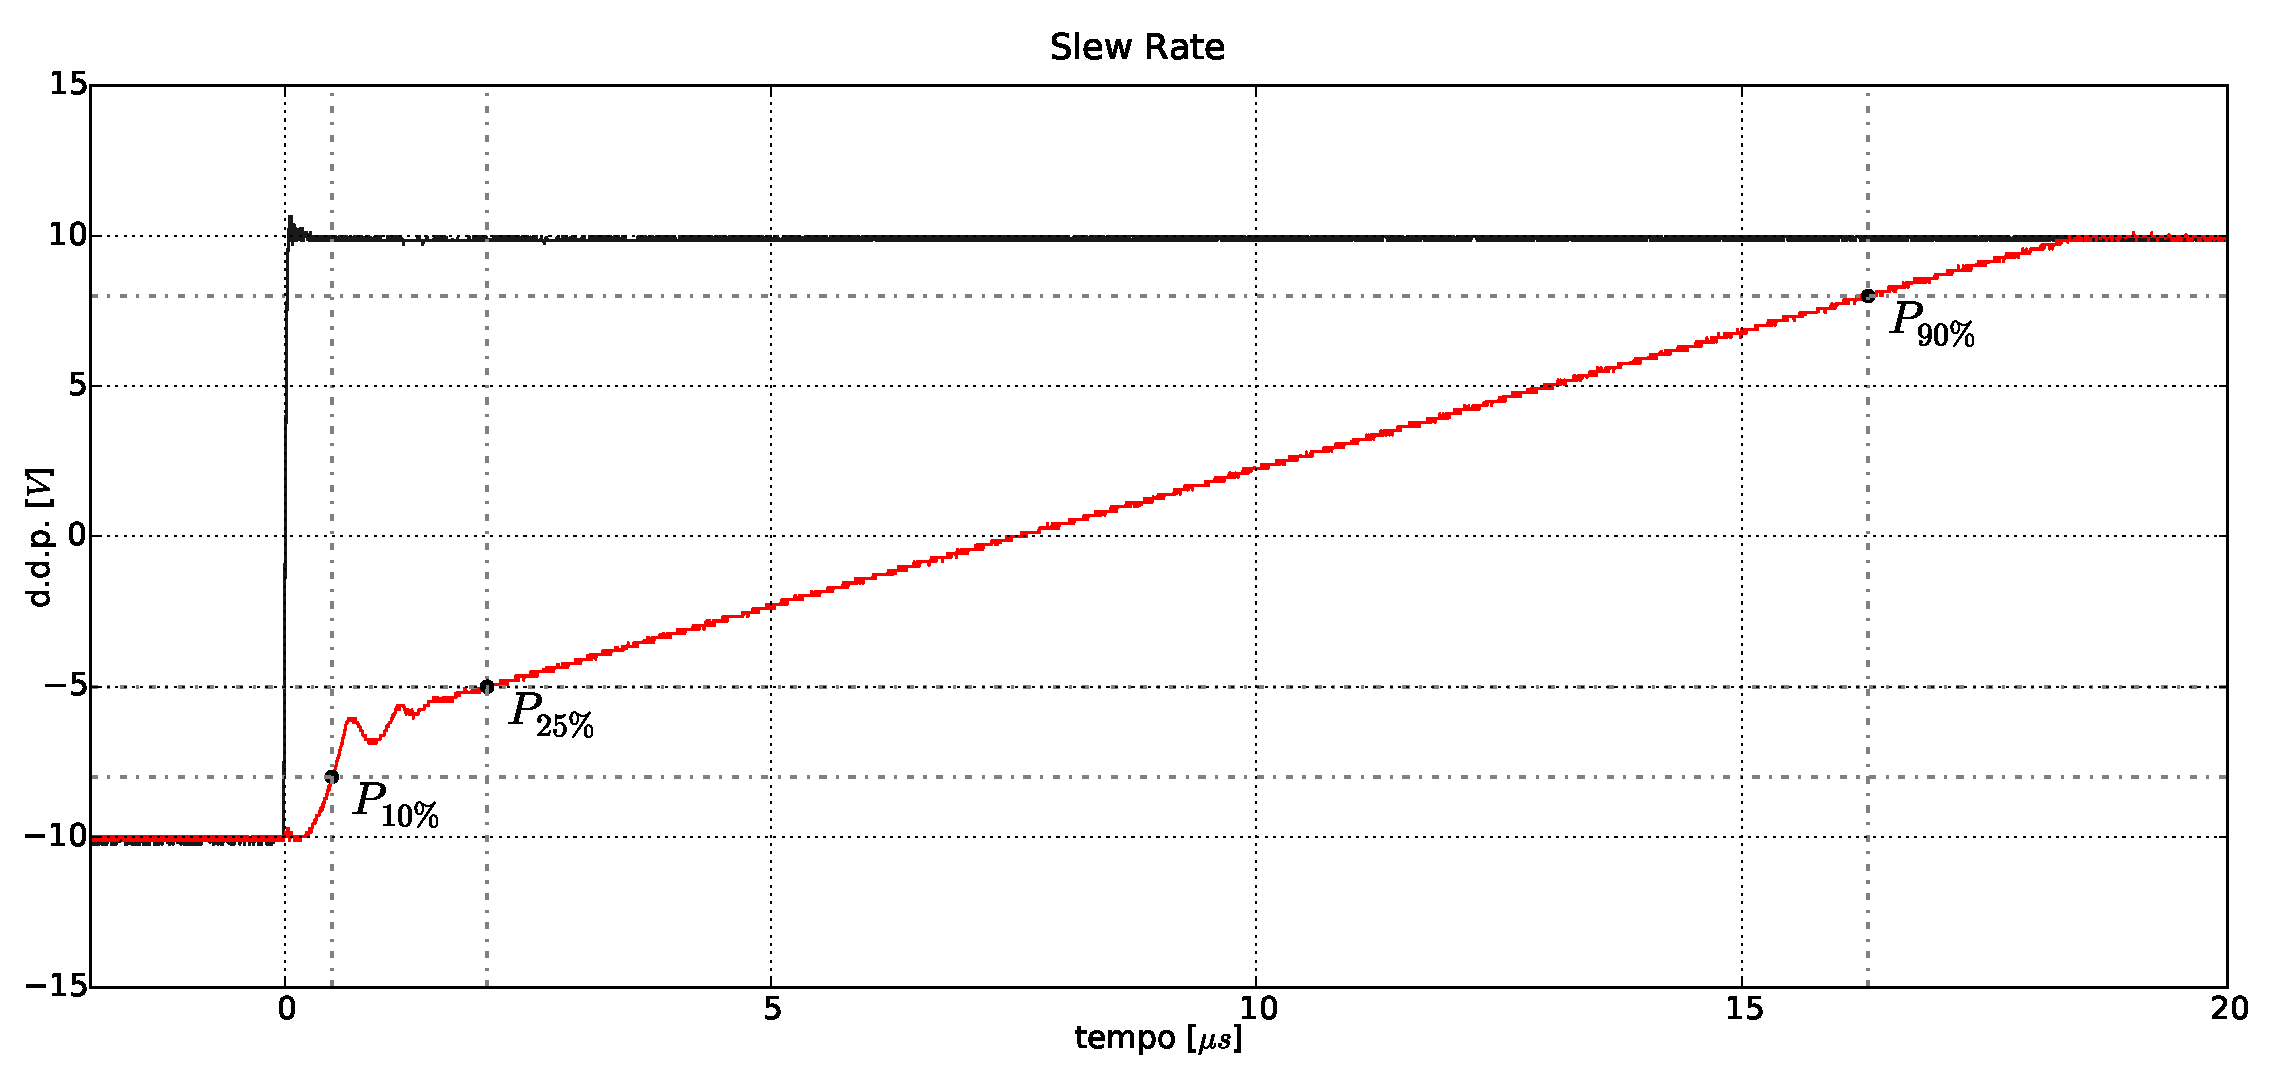
\includegraphics[width=16.5cm]{../E03/latex/sr_up.pdf}}
 \caption{Grafico della tensione in uscita (rosso) ed in entrata (nero) in funzione del tempo. I $\Delta$ sono relativi alle differenze fra le coordinate dei punti segnati.}
 \label{gr3:slew_rate}
\end{figure}

Inizialmente abbiamo posto la frequenza a $f=1$\si{\kilo\hertz} e la tensione picco picco a $V_{pp}=10$ \si{\volt}; con la funzione cursore dell'oscilloscopio abbiamo poi misurato $\Delta V = (8.07 \pm 0.01)$ \si{\volt} fra il 10\% e il 90\% del valore di tensione picco picco in uscita e la relativa $\Delta t = (15.9 \pm 0.1)$ \si{\micro\second}, ottenendo uno $SR=(0.507 \pm 0.003)$ \si{\volt\per\micro\second}.

Come però si può vedere dal grafico in Figura \ref{gr3:slew_rate} si nota che nella parte vicina al 10\% è presente una parte di segnale affetta da rumore che potrebbe rendere poco precisa la nostra misura. Infatti siamo interessati al rapporto fra i $\Delta$; dunque portare il limite inferiore ad un valore percentuale più alto, dato il rumore, rende più precisa la misura. Portando dunque la percentuale del limite inferiore al 25\% abbiamo ottenuto i seguenti valori: $\Delta V = (6.48 \pm 0.01)$ \si{\volt} e $\Delta t = (14.5 \pm 0.1)$ \si{\micro\second}, dunque $SR = (0.447 \pm 0.003)$ \si{\volt\per\micro\second}. Durante l'esperienza utilizzeremo questo valore come riferimento per lo Slew Rate del nostro amplificatore.

Abbiamo anche notato che lo Slew Rate è differente a seconda che il segnale abbia derivata $dV/dt$ positiva o negativa (grafico in Figura \ref{gr3:slew_rate_down}). Nel secondo caso, infatti, abbiamo ottenuto i seguenti valori: $\Delta V = (3.98 \pm 0.01)$ \si{\volt} e $\Delta t = (11.4 \pm 0.1)$ \si{\micro\second}, quindi $SR = (0.349 \pm 0.004)$ \si{\volt\per\micro\second}.

\begin{figure}[ht]
 \centering
   {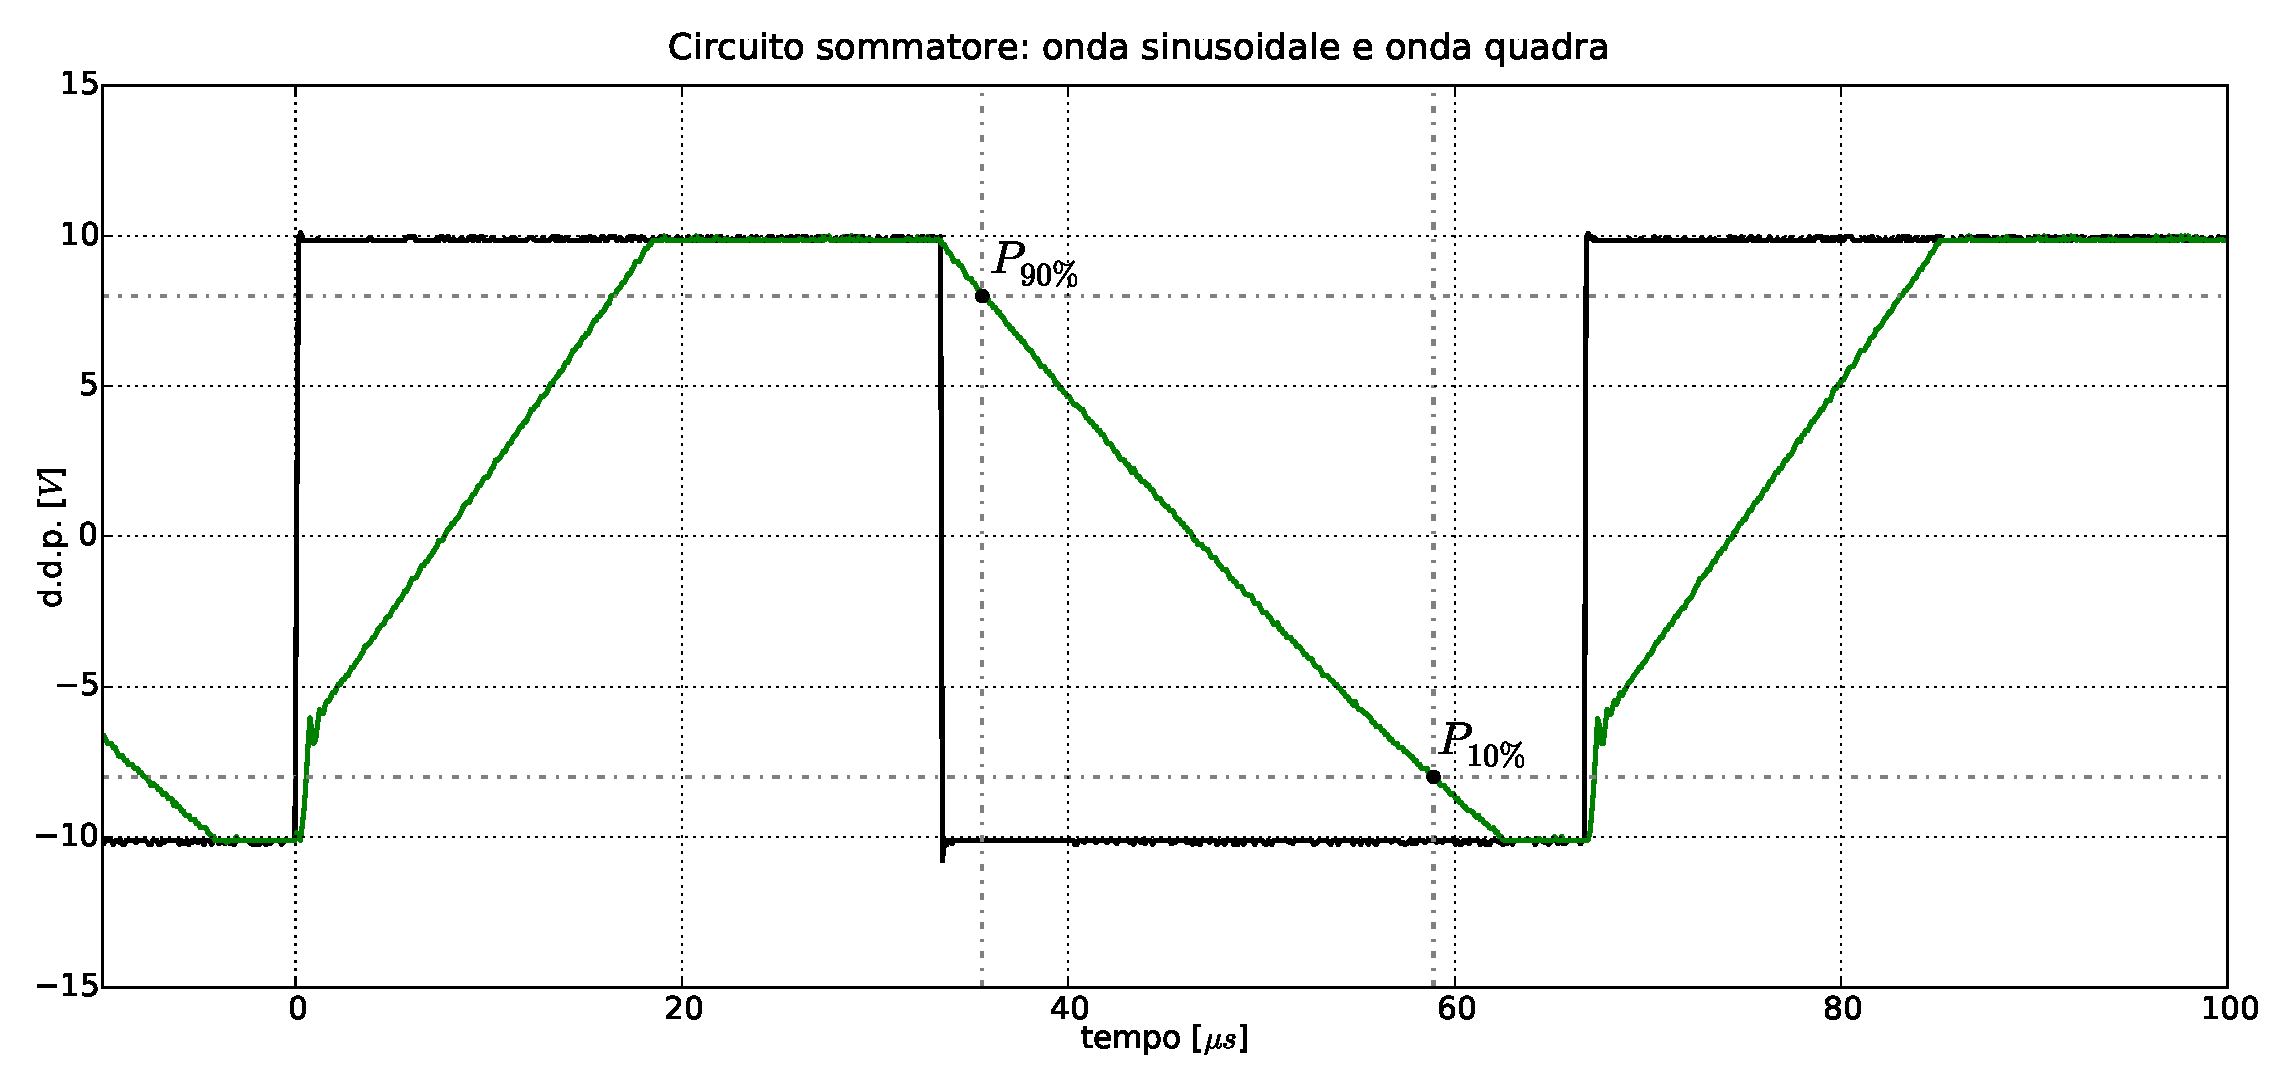
\includegraphics[width=16.5cm]{../E03/latex/sr_down.pdf}}
 \caption{Grafico della tensione in uscita (verde) ed in entrata (nero) in funzione del tempo. Osserviamo che lo slew rate sembrerebbe minore quando $dV/dt$ è minore di 0, affermazione poi confermata sperimentalmente.}
 \label{gr3:slew_rate_down}
\end{figure}